% Created 2019-04-17 wo 12:56
\documentclass[11pt]{article}
\usepackage[utf8]{inputenc}
\usepackage[T1]{fontenc}
\usepackage{fixltx2e}
\usepackage{graphicx}
\usepackage{longtable}
\usepackage{float}
\usepackage{wrapfig}
\usepackage{rotating}
\usepackage[normalem]{ulem}
\usepackage{amsmath}
\usepackage{textcomp}
\usepackage{marvosym}
\usepackage{wasysym}
\usepackage{amssymb}
\usepackage{hyperref}
\tolerance=1000
\usepackage{sectsty}
\sectionfont{\normalfont\itshape}
\subsectionfont{\normalfont\itshape}
\author{Peter van Huisstede}
\date{\today}
\title{Sum selected numbers from a list}
\hypersetup{
  pdfkeywords={},
  pdfsubject={},
  pdfcreator={Emacs 25.2.1 (Org mode 8.2.10)}}
\begin{document}

\maketitle
\begin{description}
\item[{Revision}] \$Revision: 0.2 \$
\item[{Date}] \$Date: [Time-stamp: \textit{<2019-04-17 12:56:02 (peter)>}] \$
\item[{Source}] \$Source: \emph{Users/peter/Documents/bootcamps/snippets} \$
\end{description}


\section*{Sum of all positive multiples taken from a list}
\label{sec-1}

Problem: Find the sum of all positive multiples of 3 and 5 below 1000.

\subsection*{Pencil and paper}
\label{sec-1-1}

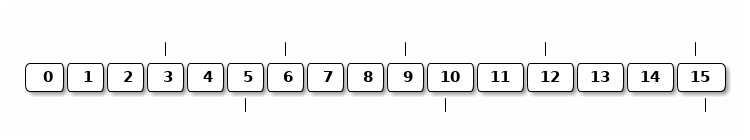
\includegraphics[width=.9\linewidth]{img/pep_sum_pos_multiples.png}

\subsection*{With the input of the pencil and paper part}
\label{sec-1-2}

We know that if we use the list [0, 1, 2, \ldots{}, 15] the result should
be 60. We also know that some of the numbers are part of both
conditions: Some multiples of 3 are also multiples of 5, for
example 15.

What we need for our program:

\begin{enumerate}
\item test for "divisible by n", here n = 3  n = 5
\item we want to keep track of the numbers that test True (for the above)
\item we want to test a lot of numbers in a non-repetitive way
\item we keep track of the hits
\item we sum our hits
\end{enumerate}

We divided our problem up into some smaller problems:

ad 1) what does 'divisible by 3' mean? It clearly does not mean that n /
   == 0.

Take 6 divided by 3 \texttt{= 2. We need to work with the remainder: 6
divided by 3 =} 2 with a remainder of 0.

There is a function to calculate the remainder of a division: \%.

6 \% 2 \texttt{= 0; 9 \% 7 =} 2

In our case, we can test for: x \% 3 \texttt{= 0 OR x \% 5 =} 0.

ad 2) If we have an empty list, we can add elements to it with the append
   function:

lst = []
lst.append(1)
lst.append(2)
lst \# [1, 2]

ad 3) Which means we want to test each number in a list twice, with the
   first test (n \% 3 \texttt{= 0) and with the second test (n \% 5 =} 0).

So we need some logic. Let's try to write this "logic" down, using pseudo-code.

\subsection*{Pseudocode}
\label{sec-1-3}

input = lst1
result = lst2

for each element of input:
    if the element \% 3 == 0:
        add the element to result
    or if the element \% 5 == 0:
        add the element to result
    otherwise: go to the next element

show the result
sum result

\subsection*{Using the REPL (iPython)}
\label{sec-1-4}

\begin{verbatim}
In [10]: input = [1, 2, 3, 4, 5, 6, 7, 8, 9, 10, 11, 12, 13, 14, 15]
In [13]: result = []
In [19]: for i in input: 
    ...:     if i % 3 == 0 or i % 5 == 0: 
    ...:         result.append(i)
In []: print(result)
Out []: [3, 5, 6, 9, 10, 12, 15]
In [21]: sum(result)                                                            
Out[21]: 60
\end{verbatim}

\subsection*{Sum}
\label{sec-1-5}

Our (first) result is another list with the positive numbers taken
from the input list that qualify as multiples of 3 or 5.

We need to calculate the sum of the elements of that list.

We could use another for-loop, something like:

sum\_result = 0
for i in result:
    sum\_result = sum\_result + i
return sum\_result

But Python already has a sum function that works with lists, so the
easy solution is:

sum(result)
% Emacs 25.2.1 (Org mode 8.2.10)
\end{document}